\section*{The Probabilistic Framework}

Our solution is based on the concept of discrete \emph{Markov processes}, which are a type of stochastic processes. A stochastic process uses probability functions to describe how a system may pass between states. In the discrete case, the system makes discrete ``jumps'' through a discrete space of states, as opposed to the continuous case where both state transitions and state space may be continuous. A Markov process is a stochastic process that satisfies the \emph{Markov property}, which states that the system's future depends only on the current state and is independent of past states. An example of a discrete Markov process is that of throwing dice and summing the results: the throws are discrete, the sum increases by a discrete amount for each throw, and the possible sums after the next throw depends only on the current sum.

In mathematical terms, the Markov property is formulated as follows (for a discrete stochastic process):
\begin{equation}
  p\left(Z_{n+1}|Z_n, Z_{n-1}, Z_{n-2}, \dots, Z_0\right) = p\left(Z_{n+1}|Z_n\right),
\end{equation}
where $Z_n$ is the system's state after step $n$ and $p\left(Z_{n+1}|Z_n, Z_{n-1}, Z_{n-2}, \dots, Z_0\right)$ is the probability that the system will assume state $Z_{n+1}$ in the next step, given that the previous states were $Z_n, Z_{n-1}, Z_{n-2}, \dots, Z_0$.

A \emph{hidden Markov model} (HMM) describes a Markov process where one cannot measure the state $Z$ of the system directly, but rather obtains an observation $u$ of the state. This observation may not be deterministic, and so we have the probability $p(u_n|Z_n)$ that we will observe $u_n$ if the current state of the system is $Z_n$.

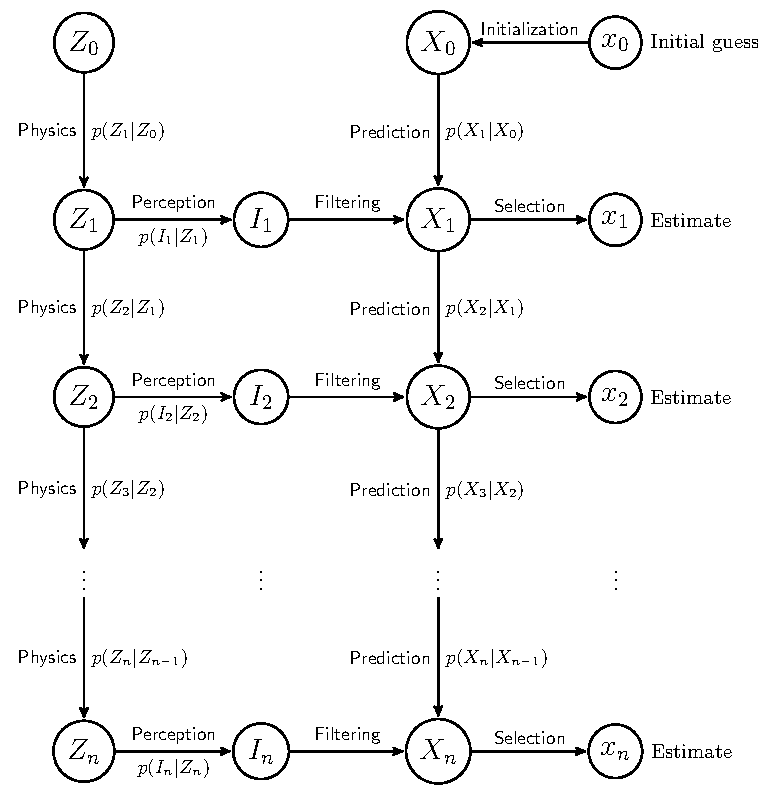
\includegraphics[width=0.2\textwidth]{figures/hmm-graph/hmm-graph.pdf}
An illustration of a Hidden Markov Model. The system assumes states $Z_1, Z_2, ...$ with probabilities $p(Z_1), p(Z_2|Z_1), \cdots$, and we obtain the observations $u_1, u_2, \cdots$ with probabilities $p(u_1|Z_1), p(u_2|Z_2), \cdots$. This is the foundation of the Particle Filter.

\subsection*{The Particle Filter}
The Particle Filter is a technique for simulating a process described by a HMM. It uses a finite set $X_n$ of hypotheses to approximate the probability function $p(Z_n)$ above. The hypotheses $X_n$ are also known as \emph{particles}, thereby the term ``particle filter''. We start with a given set $X_0$ of samples drawn from $p(Z_0)$, the probability function for the start state of the system.

TODO: Write down the state update formula that the particle filter builds upon.
